\chapter{Whitney Stratifications and pseudofibre bundles}\label{chap4}

\section{Pseudo fibre spaces}\label{chap4-sec1}\pageoriginale

The situation we with to consider is suggested by the following example. 

Let $V$ be a $\mathbb{C}$-analytic manifold with a narrow
stratification  $\{ M_i \}$ satisfying conditions (a) and (b) of
Whitney. Let $\mathscr{V}$ be the tangent bundle of $V$ and
$\mathscr{M}_i$ the tangent bundle of $M_i$.  $\mathscr{M}_i$ can be
identified naturally with a subset of $\mathscr{V}$, and let
$\mathscr{V}' = \cup \mathscr{M}_1$. $\mathscr{V}'$ consists of vectors at
points $x \in V$ which are  tangent to the $M_i$ containing
$x$. $\mathscr{V}'$ has a topology induced from  that of
$\mathscr{V}$ (under which it is not necessarily locally
compact). $\mathscr{V}'$, 
with its natural projection on $V$ is called the (complex) tangent
pseudo fibre bundle (or pseudo bundle) of the stratification.  
 
Real tangent pseudo bundles are similarly defined.
 
Remark that the homotopy lifting theorem is not in general  valid, as
shown by the following example. 
 
Let $V = S^2$ be the two dimensional sphere, and  $V = M^1_1\cup
M^2_2 \cup M^2_3$, where $M^1_1$ is a great circle and $M^2_2$,
$M^3_3$ the two (open) hemispheres of $V - M^1_1$. Let $\Gamma$ be
half of a great circle  orthogonal to $M^1_1$ as shown. Then $\Gamma$
is homotopic semicircle of $M^1_1$. This homotopy cannot be lifted to
$\mathscr{V}'$  such that in initial curve is lifted to the field of
tangent vectors\pageoriginale to $M^2_2$ orthogonal to $\Gamma$ (as
shown in the figure).  

\begin{figure}[H]
\centering{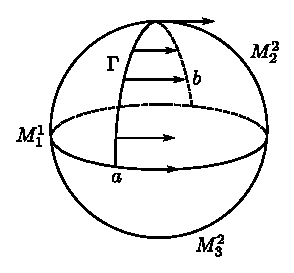
\includegraphics{vol38-figures/fig38-1.eps}}
\end{figure}

We now proceed to the general definition of a pseudo fibre space (or
pseudo fibration). 

Let $V$ be a manifold of class $C^1$ and dimension $N$. Let $\{ M_i \}$
be a narrow stratification of $V$ into connected $C^1$ locally closed
submanifolds $M_{i}$ such that each $\bar{M}_{i}$ is a union of strata
and suppose that $\{M_{i}\}$ is a locally finite family.

Let $\mathscr{K}$ be a triangulation of $V$ consistent with the above
stratification, i.e. each open simplex $K_i$ is contained in  $M_j$
for some $j$, and suppose that the open simplices  are $C^1$
submanifolds of $V$. We suppose that the following fineness condition
is satisfied. 

$(\ast)$ \textit{If} $K_j \subset M_i$ \textit{then} $\overline{K}_j
\cap \dot{M} _{i}$ \textit{is a single closed simplex}
$\overline{K}_h$ \textit{contained in the boundary}
$\dot{K}_j$ \textit{of} $K_j$ (\textit{unless}
$\overline{K}_j \cap \dot{M}_i = \emptyset$).  

This condition can always be ensured by passing to a sufficiently fine
barycentric subdivison of $\mathscr{K}$. 

Finally we suppose given a piecewise differentiable cell decomposition
$\mathscr{D} = (D_i)$ of $V$ (into open cells $D_i$; the decomposition
is not consistent with $(M_i)$) which is dual to  $\mathscr{K}$. This
dual cell decomposition is obtained as follows. If $\mathscr{K}$ is a
simplicial complex whose support $V$ is a combinatorial manifold, let
$\mathscr{K}_1$ be the 
barycentric subdivision of $\mathscr{K}$. Let $p_i$ be the barycentre
of $K_i \in \mathscr{K}$. 
The $q$-simplices of $\mathscr{K}_1$ have for vertices the
sets $(p_{i_q},\ldots,P_{i_q})$ 
with $ K_{i_{j}} \supset \overline{K}_{i_{j+1}}(j = 0,\ldots, q-1)$;
we denote this $q$-simplex by  
$(p_{i_{0}},\ldots,p_{i_{q}})$\pageoriginale and call $p_{i_{0}}$ the first, and
$p_{i_{q}}$ the last vertex. 
We have $K_{i_{q}} = \bigcup (p_{i_{0}},\ldots,p_{i_{q}})$, the union
being over those simplices 
with $p_{i_{q}}$ as last vertex. For any $i$, let
$$
D_i = \bigcup (p_i, p_{i_{1}},\ldots,p_{i_{q}})
$$
the union being taken over all the simplices
$(p_{i},\ldots,p_{i_{q}})$ of $\mathscr{K}_{1}$ for which $p_{i}$ (the
barycentre of $K_{i}$) is the first vertex. Then, if $V$ is a
combinatorial manifold of dimension $N$, each $D_{i}$ is a cell and if
$K_{i}$ has dimension $k$, $D_{i}$ is of dimension $N-k$. Further
$D_{i}$ is a cell decomposition of $V$ and has the following two
properties: 
\begin{enumerate}[(i)]
\item Each $K_{i}$ of dimension $k$ meets exactly one $D_{j}$ of
  dimension $N-k$ (viz. the $D_{i}$ described above).

\item If $K_{i}\cap D_{j}\neq \emptyset$, then $\dim(K_{i}\cap
  D_{j})=\dim K_{i}+\dim D_{j}-N$. The definitions that we now give
  will depend, {\em a priori}, on $\mathscr{K}$ and
  $\mathscr{D}$. Note also that we could give the definitions below
  when $V$ is a manifold with boundary and $\mathscr{K}$ is a cell
  decomposition. 

We begin with a lemma.
\end{enumerate} 

\setcounter{lemma}{0}
\begin{lemma}\label{chap4-lem1} % lem 1
  Given $K_i \subset M^k$,  the strata which meet the closed simplex
  $\overline{K}_i$ can be arranged so that they give rise to a sequence
\begin{equation*}
\overline{M}_1 \subsetneqq \ldots \subsetneqq
  \overline{M}_{h}=\bar{M}^k, \dim M_{j+1} > \dim M_j.\tag{1}\label{chap4-eq1}  
\end{equation*}

  Further $\overline{K}_i \cap \overline{M}_j$ form a strictly
  increasing sequence of simplices 
\begin{equation*}
\overline{K}^1 \subsetneqq\ldots\subsetneqq \overline{K}^h =
  \overline{K}_i.\tag{2}\label{eq2}  
\end{equation*}
\end{lemma}

\begin{proof} %
  Because\pageoriginale of the fineness condition, it is sufficint to prove
  \eqref{chap4-eq1}. Let $M^q$, $M^{q'}$, $q \neq q'$ be distinct strata of dimensions
  $q$, $q'$ respectively (with $q \geq q'$) meeting $\bar{K}_{i}$. If
  $q=k$, then $M^{q}=M^{k}\subset K_{i}$; hence $M^{q'}\cap
  \bar{M^{q}}\neq \emptyset$, and hence $\bar{M^{q'}}\subset
  \bar{M^{q}}$; since $M^{q}$, $M^{q'}$ are distinct, we have $q'<q$.

If $q\leq k-1$, then $M^{q}\subset \dot{M}^{k}$, $M^{q'}\subset
\dot{M}^{k}$. By our fineness condition, there is a simplex $K\subset
M^{k'}$, $k'<k$ such that $\dot{M}^{k}\cap \bar{K}_{i}=\bar{K}$. Thus,
we may replace $k$ by $k'<k$. Proceeding thus, we reach a $K'$ lying
in a stratum $M^{l}$ of dimension $l=q$ and the previous argument
applies. 


In the whole of this chapter, we suppose that $\mathscr{K}$,
$\mathscr{D}$ are given satisfying the hypotheses made above. 

The local coordinates (or charts) of our pseudo-fibration will be
defined on subsets of the following type. 

Let $\bar{K}$ be a closed simplex of $\mathscr{K}$ and $K^{0}$ one of
its vertices. Let
\begin{equation*}
L=\bar{K}\cap \overset{\circ}{\St}(K^{0})\tag{3}\label{eq3}
\end{equation*}
where $\overset{\circ}{\St}(K^0)$ is the open star of $K^{0}$ in
  $\mathscr{K}$. If $K^0 \in M^p$, then, by Lemma \ref{chap4-lem1}, 
\begin{equation*}
L=\bigcup^{k}_{q=p}L\cap M^{q}\quad\text{(where~~ $K\subset
  M^{k}$),}\tag{4}\label{eq4} 
\end{equation*}
$M^q$ being, as usual, a stratum of
  dimension $q$. 



We\pageoriginale suppose given, for each dimension $k$ such that there
is an $M^{k}\neq \emptyset$, $0\leq k\leq N$, a fibre type $F_{k}$,
i.e. a locally compact topological space $F_{k}$. We suppose that if
$h\leq k$, we are given a family $\mathscr{M}_{k,h}$ of continuous
injections $\mu_{kh}:F_{h}\to F_{k}$; we suppose that this family of
  injections is non-empty if $F_{h}$, $F_{k}$ are. We suppose that for
  $h\leq k\leq l$, and $\mu_{kh}\in \mathscr{M}_{kh}$, $\mu_{lk}\in
  \mathscr{M}_{lk}$, we have $\mu_{lk}\circ \mu_{kh}\in
  \mathscr{M}_{lh}$.

We now construct the models for our pseudo-fibrations on sets of the
type $L$ (in \eqref{eq3} above).

Let
$$
L=\bar{K}\cap \St^{0}(K^{0})=\bigcup^{k}_{q=p}L\cap M^{q}.
$$

We find $\mu_{q}\in\mathscr{M}_{kq}$ (when $L\cap M^{q}\neq
\emptyset$), such that $\mu_{k}=\id_{F_{k}}$ and if
$\alpha_{q}=\mu_{q}(F_{q})$, then $\alpha_{q'}\subset \alpha_{q}$ if
$q'\leq q$ (so that $\alpha_{q}\subset \alpha_{k}=F_{k}$); further, we
suppose that if $q'\leq q$, there is $\mu_{qq'}\in\mathscr{M}_{qq'}$
such that $\mu_{q'}=\mu_{q}\circ \mu_{qq'}$. Let
\begin{equation*}
\mathscr{L}=\bigcup^{k}_{q=p}(L\cap
M^{q})\times\alpha_{q}:\tag{5}\label{eq5} 
\end{equation*}
then
$$
L\times \alpha_{q}\subset \mathscr{L}\subset L\times F_{k}
$$
and we put on $\mathscr{L}$ the topology induced from that of $L\times
F_{k}$. 
\end{proof}

\begin{remark*} %rem 
It would be possible to work with sets $L'=\bar{L}\cap \St(K^{0})$,
where $\St(K^{0})$ is the closure of $\St^{0}(K^{0})$, instead of the
sets $L$ above in view of our fineness condition.
\end{remark*}

\setcounter{definition}{0}
\begin{definition}\label{chap4-defi1} %def 1
A\pageoriginale pseudo-fibre space, or a pseudo-fibration $\xi$ on a
$C^1$ manifold $V$ with the data of a stratification, a triangulation
and a dual cell decomposition as above is a hausdorff space $\xi$ and
a projection $\bar{\omega}:\xi\to V$  (not necessarily surjective)
such that for each set $L$ as in \eqref{eq3}, there is a homeomorphism
$g$ of $\mathscr{L}$ onto $\xi(L)=\overline{\omega}^{-1}(L)$. The pair
$(g,\mathscr{Z})$ is called a chart of $\xi$.
\end{definition}

\begin{lemma}\label{chap4-lem2}
$\bar{\omega}$ is an open map.
\end{lemma}

We omit the proof (see \cite{key3})

\begin{definition}\label{chap4-defi2} %def 2
  A pseudo-fibration is called a pseudo vector bundle (or
    pseudo-bundle) if each $F_k$ is a finite dimensional vactor
    space over  $\mathbb{R}$ or $ \mathbb{C}$, and $\mathscr{M}_{kh}$
    consists of all linear injections  of $F_h$ into $F_k$.  
\end{definition}

Let $\xi$ be a pseudo-bundle such that $F_K = \mathbb{R}^k$
(\resp $F_{2k} =  \mathbb{C}^k, M^{2k+1}\break = \emptyset$). Let $W_{r,k}$ be
the set of all $r$-frames in $F_k$, i.e. the set of all ordered
$r$-tuples of vectors linearly independent over $\mathbb{R}$ 
(\resp $\mathbb{C}$). of course, if $k < r$ (\resp $k < 2r$) then 
$W_{r,k}=\emptyset$.   

Let $\mathscr{M}_{r,k,h}$ be the set of injections of $W_{r,h}$ into 
$W_{r,k}$ induced by linear injections of $F_h$ in $F_k$. Then we
may construct a pseudo-fibration with $W_{r,k}$ as fibre type (and
$\mathscr{M}_{r,k,h}$ as given injections) for which charts are obtained as
follows. 

Let $(\mathscr{L},g)$ be a chart of $\xi$. Let $\alpha_{r,q}$ be
the space of $r$-frames in $\alpha_q$, and let 
$$
\mathscr{L}_r = \bigcup_{q} ( L \cap M^q ) \times \alpha_{r,q}.
$$   
 
Let\pageoriginale $\xi_r$ be the union $\bigcup_{x \in V}  \xi_r
(x)$, $\xi_r(x)$  being the space of $r$-frames in
$\xi(x)=\bar{\omega}^{-1}(x)$. Clearly, the map   
$$
g:\mathscr{L} \to \xi (L) 
$$
induces a bijection 
$$ 
g_r:\mathscr{L}_r \to \xi_r(L)=\bigcup_{x \in  L}\xi_{r}(x). 
$$

It is clear that there is a unique topology on $\xi_r$ making $\xi_r$
into a pseudo-fibration for which the $(\mathscr{L}_r, g_r)$  are 
charts. 

$\xi_r$ \textit{is called the associated pseudo-fibration of}
$r$-\textit{frames in} $\xi$. 

\section{Obstructions in pseudo-fibrations}\label{chap4-sec2}


Let $\xi$ be a pseudo-fibration with fibre type $F_{k}$. Let $\nu_{k}$
be the smallest integer $\nu\geq 0$ such that $\pi_{\nu}(F_{k})\neq
0$. We will make the following hypothesis: $\rho=k-\nu_{k}$ is a {\em
  positive integer independent of $k$.} (Here of course $k$ runs over
those integers with $M^{k}\neq \emptyset$ for some stratum $M^{k}$).
    
In the example given above, we have $F_{k}=W_{r,k}$; here $\rho=r-1$
in the case of real bundles, $\rho=2r-1$ in the case of complex bundles.
    
The problem we consider is that of the existence and homotopy of
continuous sections of $\xi$ (i.e. continuous maps $s:U\to \xi$,
$U\subset V$, such that $\bar{\omega}\circ s=\id_{U}.$)

\setcounter{proposition}{0}
\begin{proposition}\label{chap4-prop1} %Prop 1
The\pageoriginale obstruction dimension to skeleton-wise extension of
a section over 
$\mathscr{D}$ is $N-\rho+1$; {\em i.e.} if $\mathscr{D}^{q}$ is the
$q$-skeleton of $\mathscr{D}$, then any section $s$ of $\xi$ over
$\mathscr{D}^{N-\rho-1}$ can be extended to $\mathscr{D}^{N-\rho}$. 
\end{proposition}    

\begin{proof} %pro 
We begin by remarking that if $N\geq \rho$, every vertex $D^{0}$ of
$\mathscr{D}^{0}$ lies in a $K^{N}$, and since $N\geq \rho$,
$F_{N}\geq \emptyset$, so that a section $s$ of $\xi$ over
$\mathscr{D}^{0}$ exists if $N-\rho\geq 0$. Let $m\leq N-\rho$, and
suppose that the section $s$ is constructed on the $(m-1)$-skeleton
$\mathscr{D}^{m-1}$. To extend $s$ to $\mathscr{D}^{m}$, we choose any
$m$-cell $D^{m}$ of $\mathscr{D}^{m}$. Let $T^{n}\in \mathscr{K}\cap
\bar{D}^{m}$. We proceed by induction on $n$. We have
$T^{n}=D^{N-h+n}\cap K^{h}$, $K^{h}\subset M^{k}$; here $N-h+n\leq
m\leq N-\rho$ so that $n\leq h-\rho\leq k-\rho=\nu_{k}$. By our
induction hypothesis (on $n$) $s|\dot{T}^{n}$ is already constructed;
further, if $n=0$, $s$ can be extended to $T^{n}$. Suppose therefore
that $n\geq 1$.

Choose now an $L$ such that $\bar{T}^{n}\subset L\subset
\bar{K}^{h}\cap \St(K^{0})$. [Such an $L$ exists: there is a unique
  $K^{N-m}$ such that $D^{m}\cap K^{N-m}=T^{0}$ is a vertex. Then, by
  Lemma \ref{chap4-lem1}, $K^{N-m}\subset \bar{K}^{h}$, and we choose
  for $K^{0}$ a vertex of $\bar{K}^{h}\cap K^{N-m}$.] Consider the
chart $g:\mathscr{L}\to \xi(L)$. Then $g^{-1}s$ defines a section of
$\mathscr{L}$ on $\dot{T}^{n}$, i.e. a map $s':T^{n}\to
\alpha_{h}\subset \alpha_{k}$ (since $K^{h}\subset M^{k}$); since
$\nu_{k}\geq n$, this can be extended to a continuous map $s':T^{n}\to
\alpha_{k}$, and so gives rise to a section $g(s')=s:T^{n}\to
\xi(L)$. Proceeding thus, we obtain an extension of the section $s$ to
$\mathscr{D}^{m}$. Since this can be done for $m\leq N-\rho$, the
proposition is proved.

Before we proceed to the next proposition, we make a few remarks.

Let $I=[0,1]$, and let $\widehat{V}=V\times I$,
$\widehat{M}_{i}=M_{i}\times I$. Let $\widehat{\mathscr{K}}$ be the
{\em cell-decomposition} of $\widehat{V}$ (whose (closed) cells are
the sets $\bar{K}_{i}\times\{0\}$,\pageoriginale
$\bar{K}_{i}\times\{1\}$, $\bar{K}_{i}\times I$. Let
$\widehat{\xi}=\xi\times I$ and
$\widehat{\bar{\omega}}=\bar{\omega}\times \id_{I}$. We define the
structure of pseudo-fibration (on the manifold $V$ with boundary, and
corresponding to the cell-decomposition $\mathscr{K}$; cf. remark on
page 45) on $\widehat{\xi}$ as follows. 

If $L=\bar{K}\cap \St^{0}(K^{0})\subset V$ is a set defining a chart
of $\xi$, let $\widehat{L}=L\times I$, and $\widehat{g}$ the bijection
of $\widehat{\mathscr{L}}=\mathscr{L}\times I$ onto
$\widehat{\xi}(\widehat{L})=\widehat{\bar{\omega}}^{-1}(\widehat{L})$
given by $\widehat{g}=g\times \id_{I}$. The fibre type of
$\widehat{\xi}$ and the injections between the fibres are the same as
for $\xi$.

Let $s_{N-\rho}$, $s'_{N-\rho}$ be two sections of $\xi$ over
$\mathscr{D}^{N-\rho}$, the $N-\rho$ skeleton of $\mathscr{D}$. We
identify them with sections on $\mathscr{D}^{N-\rho}\times\{0\}$,
$\mathscr{D}^{N-\rho}\times \{1\}$ respectively, of $\widehat{\xi}$. 
\end{proof}  

\begin{proposition}\label{chap4-prop2} %pro 2
Two sections $s_{N-\rho}$, $s'_{N-\rho}$ of $\xi$ on
$\mathscr{D}^{N-\rho}$ are homotopic on $\mathscr{D}^{N-\rho-1}$; in
fact a given homotopy on $\mathscr{D}^{N-\rho-2}$ can be extended to
$\mathscr{D}^{N-\rho-1}$. 
\end{proposition} 

\begin{proof} %pro
We do not consider the case when $F_{N}$ is not connected, for we
would then have $\rho>N$. If $F_{N}$ is connected, any two sections of
$\xi$ over $\mathscr{D}^{0}$ are homotopic.

Let $m\leq N-\rho-1$. By induction on $m$, suppose given a homotopy
between $s$, $s'$ on $\mathscr{D}^{m-1}$. Let $D^{m}$ be an $m$-cell
of $\mathscr{D}^{m}$. Then, with the notations as above,
$$
T^{n}=D^{N-h+m}\cap K^{h}, K^{h}\subset M^{h}; N-h+n\leq m\leq N-\rho-1
$$
so that
$$
\nu_{k}\geq n+1\geq 1.
$$

This\pageoriginale implies that $F_{k}$ is connected, so that (if
$n=0$) any two sections on $T^{0}$ are homotopic. Suppose (by
induction on $n$) that, for $n\geq 1$, the homotopy between $s$, $s'$
on $\mathscr{D}^{m-1}$ is extended to all the $T^{\lambda}\subset
\bar{D}^{m}$ for which $\lambda<n$. Then $s$ on $T^{n}\times \{0\}$,
$s'$ on $T^{n}\times \{1\}$ and the given homotopy on
$\dot{T}^{n}\times I$ define a section of $\widehat{s}$ on the whole
boundary of $T^{n}\times I$ and we have only to show that this section
can be extended to $\bar{T}^{n}\times I$.

To prove this, we choose $L$ with $\bar{T}^{n}\subset L\subset
\bar{M}^{k}$ and a chart $\widehat{g}:\widehat{\mathscr{L}}\to
\widehat{\xi}(\widehat{L})$ as above. Clearly
$\widehat{g}{}^{-1}\widehat{s}$ is a section of
$\widehat{\mathscr{L}}$ on the boundary of $T^{n}\times I$, hence
gives rise to a map of the boundary of $T^{n}\times I$ into
$F_{k}$. Since $k\geq h\geq n+\rho+1$, so that $\nu_{k}\geq n+1$, this
can be extended to a map of $\bar{T}^{n}\times I$ into $F_{k}$, and so
gives rise to a section of $\widehat{\mathscr{L}}$ on
$\bar{T}^{n}\times I$, and its image by $\widehat{g}$ is a section of
$\widehat{\xi}$ on $\bar{T}^{n}\times I$ extending $\widehat{s}$. This
proves that the given homotopy on $\mathscr{D}^{m-1}$ can be extended
to $\mathscr{D}^{m}$ if $m\leq N-\rho-1$. The proposition follows.
\end{proof}

\begin{proposition}\label{chap4-prop3} %pro 3
Suppose $F_{p}\neq \emptyset$ and $K^{0}\in M^{p}$. Then $\xi$ has a
section on the open star $U$ of $K^{0}$ in $\mathscr{K}$. Moreover, if
$F_{p}$ is arcwise connected, any two sections over $U$ are homotopic.
\end{proposition}

\begin{proof} % pro
To construct a section $s$ on $U$, we proceed by induction on the
dimension $h$ of simplices $K^{h}\subset U$. Clearly, since $F_{p}\neq
\emptyset$, $s|K^{0}$ exists. Suppose $s|K^{l}$ given for all $l<h$,
and $K^{h}\subset U\cap M^{k}$, $L=U\cap \bar{K}^{h}$. Consider a
chart $g:\mathscr{L}\to \xi(L)$. We are given a section of $\xi$ on
$\dot{L}\cap U$, hence a section of $\mathscr{L}$ on $\dot{L}\cap U$,
a fortiori  a map of $\dot{L}\cap U$ into $F_{k}$. Since $\dot{L}\cap
U$ is a hemisphere on the boundary\pageoriginale of $L$, this can be
extended to a map $L\to F_{k}$. Since the interior of $L$, which is
$K^{h}$, has the property that $K^{h}\times F_{k}\subset \mathscr{L}$,
this gives us a section of $\mathscr{L}$ on $L$ extending the given
section on $L\cap U$, and the image by $g$ gives us a section of $\xi$
on $L$ extending the given section on $\dot{L}\cap U$.

Suppose now that $F_{p}$ is connected. We use the notation before
Proposition \ref{chap4-prop2}. Given sections $s_{0}$, $s_{1}$ of
$\widehat{\xi}$ on $U\times\{0\}$ and $U\times\{1\}$, we have to
extend it to a section $\widehat{s}$ of $U\times I$. Let $K^{h}\times
I\subset U\times I$ and suppose $\widehat{s}$ given on $K^{l}\times I$
for all $l<h$. Let $K^{h}\subset U\cap M^{k}$, $L=U\cap \bar{K^{h}}$
and let $\widehat{g}:\widehat{\mathscr{L}}\to
\widehat{\xi}(\widehat{L})$ be a chart. As before, this leads to a map
of $L\times \{0\}\cup L\times\{1\}\cup (\dot{L}\cap U)\times I$ into
$F_{k}$, and if $h\geq 1$, this union is not the whole of the boundary
of $L\times I$, and the map therefore extends to $L\times I$, which,
as before gives us a section of $\widehat{\xi}$ on $L\times I$
extending $s_{0}|L\times\{0\}$ and $s_{1}|L\times \{1\}$ (and the
section defining the homotopy on $L\times I$). If $h=1$, since $F_{p}$
is arcwise connected, the problem is trivial. Our proposition follows
by induction on $h$. 
\end{proof}

\section{Local structure of pseudo vector bundles}\label{chap4-sec3}

Let $\{M_{i}\}$ be a stratification of the complex manifold $V$. Let
$\xi$ be a topological space $\bar{\omega}:\xi\to V$ a continuous map
such that for $x\in M^{k}$, $\bar{\omega}^{-1}(x)$ is homeomorphic to
$F_{k}=\mathbb{C}^{k}$. We look for conditions that
$\bar{\omega}:\xi\to V$ be a pseudo-fibration. We shall apply these
considerations to the tangent fibration of a Whitney stratification in
\S \ref{chap4-sec4}.

In\pageoriginale this section, if $K_{i}\subset M^{p}$, we write
${}_{p}K_{i}$ or simply ${}_{p}K$ for $K_{i}$. Let
${}_{p}U=\St^{0}({}_{p}K)$ and
$\widetilde{U}_{p}=\overline{{}_{p}U}\cap \bigcup_{q\geq p}M^{q}$. 

The conditions that we impose on our space $\xi$ are the following.

$\Phi_1$. To each ${}_PK \subset M^p$, we can associate a non-empty
family $\Phi(p)$ of mappings               
$$ 
\varphi_p:\widetilde{U}_p \times F_p \to \xi
(\widetilde{U}_p)=\bar{\omega}^{-1} (\widetilde{U}_p) 
$$            
such that $\varphi_p$ is continuous, and $\varphi_p\mid \{x\}\times F_p$
is a $\mathbb{C}$-linear injection into $\xi(x)$. 

$\Phi_2$.~ Suppose that ${}_PK \subset \overline{{}_{m}K}, {}_mK \subset
M^{m}$, $p \leq m$. Then, clearly, $\overline{{}_{p}U}\supset
\overline{{}_{m}U}$, and $\widetilde{U}_{p}\supset \widetilde{U}_{m}$.
              
Let $\mu$ be a linear injection of $F_{p}$ in $F_{m}$. Then, given a
$\varphi_{p}$ as in $\Phi_{1}$, there is a $\varphi_{m}\in \Phi(m)$
$$
\varphi_{m}:\widetilde{U}_{m}\times F_{m}\to \xi(\widetilde{U}_{m})
$$ 
such that
$$
\varphi_{p}\mid \widetilde{U}_{m}\times
F_{p}=\varphi_{m}(\id_{\widetilde{U}_{m}}\times \mu),
$$
i.e.\quad $\varphi_{p}(x,\zeta)=\varphi_{m}(x,\mu(\zeta))$ for
$x\in\widetilde{U}_{m}$, $\zeta\in F_{p}$. 

\begin{proposition}\label{chap4-prop4} %pro 4
If $\xi$ is a topological space with a map $\bar{\omega}:\xi\to V$ for
which a family of maps $\{\varphi\}=\{\Phi(p)\}_{p\geq 0}$ satisfying
$\Phi_{1}$ and $\Phi_{2}$ exist, then $\xi$ carries a natural
structure of pseudo-vector bundle.
\end{proposition} 
   
\begin{proof} %pro 
It\pageoriginale is clearly sufficient to construct charts for
$\bar{\omega}:\xi\to V$. 

Let $L=\bar{K}^{m}\cap \St^{0}(K^{0})$, $K^{0}\in M^{p}$,
$K^{m}\subset M^{k}$.

Let $\alpha_{p}\subset\ldots\subset \alpha_{k}=F_{k}$ be a family of
subspaces of $F_{k}=\mathbb{C}^{k}$ such that $\alpha_{q}\approx
F_{q}$, and let
$$
\mathscr{L}=\bigcup^{k}_{q=p}(L\cap M^{q})\times\alpha_{q}\subset
L\times F_{k}. 
$$

Let $\pi_{F}$, $\pi_{L}$ be the projections of $\mathscr{L}$ into
$F_{k}$, $L$ respectively. Let $e_{1},\ldots,e_{k}$ be a $k$-frame in
$F_{k}$ such that $e_{1},\ldots,e_{q}\in F_{q}$ (and so span
$F_{q}$). By our fineness condition, there exists, for each $q$, a
$q^{K}=K^{h}$ such that
$$
K^{h}\subset L\cap M^{q}\subset \bar{K}^{h},\quad\text{i.e.}\quad
q^{K}\subset L\cap M^{q}\subset \overline{{}_{q}K}.
$$

Thus
$$
\pi^{-1}_{F}(\alpha_{q})=\bigcup_{h\geq q}(L\cap
M^{h})\times\alpha_{q}=(L\cap \bigcup_{h\geq
  q}M^{h})\times\alpha_{q}=(L\cap \widetilde{U}_{q})\times \alpha_{q}.
$$

We will construct an isomorphism $g:\mathscr{L}\to \xi(L)$ inductively
by constructing maps
$$
g_{q}:\pi^{-1}_{F}(\alpha_{q})\to \xi(L\cap \widetilde{U}_{q}).
$$

When $q=p$, $\pi^{-1}_{F}(\alpha_{q})=(L\cap \widetilde{U}_{p})\times
\alpha_{p}$; now, by $\Phi_{1}$, there is a map
$$
g_{p}:\pi^{-1}_{F}(\alpha_{p})\to \xi(L\cap \widetilde{U}_{p}),
$$
which is the restriction to $L\cap \widetilde{U}_{p}$ of a map
$\widetilde{U}_{p}\times \alpha_{p}\to \xi(\widetilde{U}_{p})$. 
$g_{p}$ is an injection on each fibre $\{x\}\times \alpha_{p}$. Now
suppose that
$$
g_{q}:\pi^{-1}_{F}(\alpha_{q})\to \xi(L\cap \widetilde{U}_{q})
$$\pageoriginale
is determined as the restriction to $L\cap \widetilde{U}_{q}$ of a map
$\varphi_{q}:\widetilde{U}_{q}\times \alpha_{q}\to
\xi(\widetilde{U}_{q})$. Let $h$ be the smallest integer $>q$
occurring among the $\alpha_{q},\ldots,\alpha_{k}$. By $\Phi_{2}$,
there is a map $\varphi_{h}:\widetilde{U}_{h}\times \alpha_{h}\to
\xi(\widetilde{U}_{h})$ such that
$\varphi_{h}|\widetilde{U}_{h}\times\alpha_{q}=\varphi_{q}\mid\widetilde{U}_{h}\times\alpha_{q}$;
we may take $g_{h}=\varphi_{h}\mid L\cap \widetilde{U}_{h}$. This
gives us finally a map $g$ of $\mathscr{L}=\cup
\pi^{-1}_{F}(\alpha_{q})$ into $\xi(L)$ which is injective on the
fibres. Since the fibres of $\mathscr{L}$ and $\xi(L)$ at any point
have the same dimension, $g$ is an isomorphism.
\end{proof}

\begin{remark*}
If $\xi$ is a complex pseudo vector bundle as above, two mapping
$\varphi_{p}$, $\varphi'_{p}\in\Phi(p)$ [cf. $\Phi_{1}$] are isotonic,
i.e. there is a continuous family $\varphi_{p}(t)$, $0\leq t\leq 1$ of
maps in $\Phi(p)$ on ${}_{p}U$ with $\varphi_{p}(0)=\varphi_{p}$,
$\varphi_{p}(1)=\varphi'_{p}$. 
\end{remark*}

If ${}_{p}K=K^{0}\in M^{p}$ is a vertex, we remark, using a chart,
that $\varphi_{p}$, $\varphi'_{p}$ correspond to sections of the
associated bundle $\xi_{p}$ of $p$-frames over ${}_{p}U$, and two such
sections are homotopic by Proposition \ref{chap4-prop3}.

In the general case, one proceeds by induction, as in the proof of
Proposition \ref{chap4-prop3}.

\section[Pseudo-fibration corresponding to a Whitney
  stratification]{Pseudo-fibration corresponding to a Whitney\hfill\break
  stratification}\label{chap4-sec4} 
 
We prove in this section the following
   
\begin{theorem*} %the 
Let $\{M_{i}\}$ be a Whitney stratification of a complex manifold $V$
and $\mathscr{V}'$ the space of tangent vectors to the strata {\em (see
  beginning of \S \ref{chap4-sec1})}. Then $\mathscr{V}'$ carries a
natural structure of pseudo-vector bundle.
\end{theorem*}
 
\begin{proof} %
By\pageoriginale the triangulation theorem for analytic sets, there is
a triangulation $\mathscr{K}$ of $V$ compatible with $\{M_{i}\}$. We
suppose (by suitable subdivision) that $\mathscr{K}$ satisfies the
fineness condition of \S \ref{chap4-sec1} (Condition (*) on p.~45),
and that the open star of any simplex is contained in a coordinate
neighbourhood of $V$.

Let $K^{l}\subset M^{p}$ ($p$ is the complex dimension of
$M^{p}$). Then, by the finenss condition, there is a vertex $K^{0}$ of
$\bar{K}^{l}$, $K^{0}\in M^{p}$. Then $\widetilde{U}_{l}\subset
\widetilde{U}_{0}$, and we shall construct the maps $\varphi\in
\Phi(p)$ on $\widetilde{U}_{0}\times\mathbb{C}^{p}$,
i.e. $\varphi:\widetilde{U}_{0}\times \mathbb{C}^{p}\to
\mathscr{V}'(\widetilde{U}_{0})$. This means, of course, that there is
a continuous field of $p$-frames in $\widetilde{U}_{0}$ compatible
with the stratification; further, since $K^{0}$ is a vertex,
$\widetilde{U}_{0}$ is the star of $K^{0}$. 

We will use the following lemma; its proof is to be found in
\cite{key5}. 
\end{proof}

\setcounter{lemma}{1}                 
\begin{lemma}\label{chap4-sec4-lem2} %lem 2
Let $X$ be a Euclidean complex, $Y$ a subcomplex. Then $Y$ has a
fundamental system of tubular neighbourhoods $\Theta$ in $X$ such that
the segments $]y,\dot{x}]$, $y\in Y$, $\dot{x}\in\Theta$, form a
    partition of $\Theta-Y$.
 \end{lemma}
 
We consider a Euclidean complex homeomorphic to $\mathscr{K}$; we use
the same notation in this euclidean complex as in $V$. Let $U=U_{0}$
be as above; let $\dot{U}$ be its boundary and $M_{j}$ a stratum of
dimension $>p$ with $\dot{M}_{j}\cap U\neq \emptyset$. Consider the
subcomplex $X=\bar{M}_{j}\cap \dot{U}$ of $\dot{U}$, and the
subcomplex $Y=\dot{M}_{j}\cap \dot{U}$ of $X$. Let $\Theta$ be a
tubular neighbourhood as in Lemma \ref{chap4-sec4-lem2}, and $t\in [0,1]$
the parameter for the directed segment $[y,x]$ (parametrized
linearly). For $u\in[0,1]$, let $\lambda_{u}$ be the homothesy having
$y_{0}=K^{0}$ as centre, the dilatation being $u$. 
Let\pageoriginale $T$ be the complex generated by the
$\lambda_{u}(\Theta)$, $0\leq u\leq 1$, and let $y_{u}=\lambda_{u}(y)$
(and similr notation for other points). clearly, the segments
$]y_{u},x_{u}]$ form a partition of $T-\dot{M}_{j}\cap \dot{U}$. $T$
    is called a ``conical neighbourhood'' of $\dot{M}_{j}\cap \dot{U}$
    in $\bar{M}_{j}\cap \dot{U}$. $T$ is called a ``conical
    neighbourhood'' of $\dot{M}_{j}\cap \dot{U}$ in $\bar{M}_{j}\cap
    \dot{U}$. We also speak of conical neighbourhoods in $\mathscr{K}$
    on the original manifold $V$. Remark it is not a real
    neighbourhood since it is not a neighbourhood at $K^{0}$.

We now proceed to the construction of a field of $p$-frames in
$\widetilde{U}$. We may suppose that $V$ is an open set in
$\mathbb{C}^{N}$ because of our hypothesis that the star of any
simplex is contained in a co-ordinate neighbourhood.

If $K^{0}\in M^{p}$ with $p=0$, the statement is trivial; let then
$p\geq 1$. Let $y_{0}=K^{0}\in M^{p}=M$. Let $e_{i}(y_{0})$, $1\leq
i\leq p$ be a basis of $T(M,y_{0})$. We shall extend the $p$-frame
$Z=\{e_{i}(y_{0})\}$ to the complexes $M^{q}_{j}\cap \widetilde{U}$ by
induction on $q=\dim M^{q}_{j}$. Suppose this to be done for all
$M^{q}_{j}$ of dimension $q<m$, and let $N$ be a stratum of dimension
$m$ such that $N\cap \bar{U}\neq \emptyset$. We suppose furthermore
that all the vectors already constructed on $M^{q}_{j}\cap
\widetilde{U}$ tend to zero at a point of $\bar{U}-\widetilde{U}$
which is subcomplex of $\dot{U}$ by the definition of
$\widetilde{U}$. For a point $x$ in the closure of the complement of
the conical neighbourhood $T$ of $\dot{N}\cap \bar{U}$ in $N\cap
\bar{U}$, let $e_{i}(x)$ be the orthogonal projection (with respect to
the metric induced on $U$ from $\mathbb{C}^{N}$) on the tangent space
$T(N,x)$ of the translate of $e_{i}(y_{0})$ to $x$. If $x\in T$,
$x\notin \dot{N}$, then $x$ is on a unique segment $[y,x_{1}]$
corresponding to parameter value $t\in[0,1]$.     
Let\pageoriginale $\xi(x)$ [\resp $\eta(x)$] be the projection on
$T(N,x)$ of the translate of $e_{i}(x)$ [\resp $e_{i}(y)$]. (Note
that, by induction, the $e_{i}$ are defined on $\dot{N}\cap
\widetilde{U}$). We have already supposed that these can be extended
to $\dot{N}\cap \bar{U}$ and vanish on $\bar{U}-\widetilde{U}$). We
set
$$
e_{i}(x)=t\xi(x)+(1-t)\eta(x).
$$

The field $e_{i}$ is continuous on $N\cap \bar{U}$ (it may have
zeros). We prove that it is continuous on $\bar{N}\cap \bar{U}$. Let
$y\in\dot{N}\cap \bar{U}$, and let $y\in M_{j}$. {\em In fact, by
  Whitney's condition (a),} if $x$ is near $y$, then the orthogonal
projection $v=\eta(x)$ of the translate of $e_{i}(y)\neq 0$ to $x$ on
$T(N,x)$ is near $v$. In fact, if this were not true, we could find a
sequence of points $x_{i}\in N$ tending to $y$ such that (the
Grassmannian being compact) $\kappa T(x_{i},N)$ converges to a
limit $\kappa T$ such that $T$ is transverse to $T(y,M_{j})$; this is
impossible since our stratification is, by assumption, a Whitney
stratification. Since, as $x$ tends to $y$, the parameter value tends
to zero, $e_{i}(x)=\eta(x)+t(\xi(x)-\eta(x))$ is near the translate of
$e_{i}(y)$ to $x$.

It is clear from the above construction that we may find continuous
fields $e_{1},\ldots,e_{p}$ in $\bar{N}\cap \bar{U}$ extending the
fields on $\dot{N}\cap \bar{U}$ (which form a $p$-frame on
$\dot{N}\cap \widetilde{U}$). There is a neighbourhood $W$ of $y_{0}$
such that the $e_{i}(x)$ form a $p$-frame at $x$ for $x\in W$. By
induction, the $e_{i}(x)$ form a $p$-frame at points of $\dot{N}\cap
\widetilde{U}$. Consequently, there is a neighbourhood $T'$ of all the
points of $\dot{N}\cap \widetilde{U}$ in $\bar{N}\cap \widetilde{U}$
on which the $e_{i}$ remain a $p$-frame ($T'$ may not be a
neighbourhood in $\bar{N}\cap \bar{U}$). It is immediate that we may
take $T'\subset T$ and suppose that $\dot{N}\cap \widetilde{U}$
is\pageoriginale a retract of $T'$.


In $T''=T'\cup W$, the $e_{i}$ form a $p$-frame. Let $H=N\cap
\widetilde{U}-T''\subset N$. Moreover, if $T'$ and $W$ are suitably
chosen, then each $K^{l}\cap H$ is a cell. (This is obvious for the
euclidean complexes, and the general case can be reduced to this by a
homeomorphism.) 

We now extend the $p$-frame from $T''$ to $H$ by doing this stepwise
on the cells $K^{l}\cap H$. Let $\mathscr{T}_{p}$ be the (locally
trivial) fibre space of $p$-frames tangent to $N$. We suppose, by
induction on $l$, that the frame is extended to the complex
$\mathscr{K}^{l-1}\cap H$ and consider a cell $K^{l}\cap H$.


First suppose that $\widetilde{U}=\bar{U}$ (i.e. that $\dot{U}\cap
M^{p}=\emptyset$). In this case, $T''$ being suitably chosen,
$K^{l}\cap H$ is a hemisphere on the boundary $\dot{K}^{l}$. Hence,
the following lemma implies that any section of $\mathscr{T}_{p}$ on
$\dot{K}^{l}\cap H$ can be extended to $K^{l}\cap H$, and our result
would follow.

\begin{lemma*} %lem 
Let $\Delta$ be a convex polyhedron in $\mathbb{R}^{l}$ and
$\mathscr{T}$ a locally trivial fibre space on $\Delta$. Let $S$ be an
open linear simplex contained in $\dot{\Delta}$. Then any section of
$\mathscr{T}$ on $\dot{\Delta}-S$ can be extended to $\Delta$.
\end{lemma*}

\begin{proof} %pro 
Since the pair $(\Delta,\dot{\Delta}-S)$ is homeomorphic to the pair
$(I^{l},I^{l-1}\times\{0\})$ [$I$ being the unit interval on
  $\mathbb{R}$], we replace $\Delta$ by $I^{l}$ and $S$ by
$\dot{I}^{l}-I^{l-1}\times\{0\}$. If $s$ is a section of $\mathscr{T}$
on $I^{l-1}\times\{0\}$, by the homotopy lifting theorem (lift the
trivial homotopy of $I^{l-1}\times\{0\}$), there is a map
$F:I^{l}(=I^{l-1}\times I)\to \mathscr{T}$ with\pageoriginale $p\cdot
F(x,t)=(x,t)$ and $F(x,0)=s(x)$ [here $p:\mathscr{T}\to I^{l}$ is the
  projection]. Clearly $F$ is a section of $\mathscr{T}$ on $I^{l}$
extending $s$.
\end{proof}

In the case when $\widetilde{U}\neq \bar{U}$, let $Y=\dot{K}^{l}\cap
(\bar{U}-\widetilde{U})$. Then $Y\subset \dot{U}$. We consider a
sequence $\{Y_{\nu}\}$ of neighbourhoods of $Y$ in $K^{l}$ such that
($Y_{\nu}-Y$ is a subcomplex of a suitable subdivision of $K^{l}-Y$
and) $\bar{Y}_{\nu+1}\subset Y_{\nu}$,
$\bigcap^{\infty}_{\nu=1}Y_{\nu}=Y$. 

The argument used above shows that the given $p$-frame can be extended
to $K^{l}\cap H-Y_{\nu}$. For a suitable choice of the $\{Y_{\nu}\}$,
we can apply the lemma above to extend any section of
$\mathscr{T}_{p}$ on $K^{l}\cap H-Y_{\nu}$ to $K^{l}\cap
H-Y_{\nu+1}$. Thus, in both cases, the given $p$-frame can be extended
to $K^{l}\cap H$.

This proves that we can construct continuous $p$-frames on
$\widetilde{U}$, and $\Phi_{1}$ is proved.

To prove $\Phi_{2}$, we have only to prove that if ${}_{p}K\subset
{}_{m}\bar{K}$, ${}_{m}K\subset M^{m}$, and if $\{e_{i}\}_{1\leq i\leq
  p}$ is a continuous $p$-frame on $\widetilde{U}_{p}$, these can be
extended to an $m$-frame on $\widetilde{U}_{m}$. 

The proof is exactly similar to that given above: we choose a vertex
$y'_{0}$ of ${}_{m}\bar{K}$ in $M^{m}$, and vectors
$e_{p+1}(y'_{0}),\ldots,e_{m}(y')$ at $y'_{0}$ linearly independent of
$e_{1}(y'_{0}),\ldots,e_{p}(y'_{0})$ and apply the above reasoning;
one has to consider neighbourhoods where the fields constructed on
$\bar{N}\cap \widetilde{U}$, $\{U=\St^{0}(y'_{0})\}$ are independent
of the $e_{i}(1\leq i\leq p)$ and replace the fibre space
$\mathscr{T}_{p}$ by the space $\mathscr{T}_{p,m}(e_{1},\ldots,e_{p})$
of $m-p$ vectors which are independent of the $e_{1},\ldots,e_{p}$. 


\medskip
\noindent
{\large\bf Fields of frames tangent to a Whitney
  stratification}\pageoriginale
\smallskip

From the results of \S \ref{chap4-sec1} and the above theorem, it
follows that the $r$-frames of the fibres of $\mathscr{V}'$ form a
pseudofibre space $\mathscr{V}'_{r}$. The fibre type of
$\mathscr{V}'_{r}$ over a stratum $M^{k}$ (of complex dimension $k$)
is empty for $k\leq r$ and, for $k\geq r$, is the manifold of
$r$-frames in $\mathbb{C}^{k}$, which has the homotopy type of the
Stiefel manifold $U(k)/U(k-r)$.

Hence the first non-zero homotopy group of the fibre $F_{k,r}$ over
$M^{k}$ is $\pi_{2k-2r+1}(F_{k,r})$; hence $\rho=2r-1$. If $N$ is the
complex dimension of $V$, we deduce from the results of \S
\ref{chap4-sec2} the following

\begin{prop*} %pro 
With the notation of \S \ref{chap4-sec2}, the obstruction dimension to
skeletonwise extension, over $\mathscr{D}$, of a continuous field of
$r$-frames ``tangent to the strata'' is $2p=2(N-r+1)$. Two such
fields, defined on $\mathscr{D}^{2p-1}$, are homotopic on
$\mathscr{D}^{2p-2}$. Further, if $y_{0}\in M^{p}$, $p\geq r$, then,
on the open star of $y_{0}$ in $\mathscr{K}$, there exists a
continuous field of $r$-frames tangent to the strata.
\end{prop*}

Whitney has posed the following question: Can one find locally,
families of (real) analytic or semi-analytic fields of vectors which
are linearly independent and consistent with the stratification?

Our proposition shows that {\em continuous} fields of this kind exist.

Whitney has also shown that, in general, holomorphic fields with this
property do not exist (see \cite{key6}).

\medskip
{\large\bf Obstruction classes.}\pageoriginale
\smallskip

Let us consider first the simple example when the stratification of
$V$ consists of a (closed) submanifold $M$ of complex dimension $k$
and $M'=V-M$. Let $\mu$ be the homomorphism of $H^{i}(M,\mathbb{Z})$
into $H^{i+N-k}(V,\mathbb{Z})$ which is the Thom-Gysin isomorphism
followed by the canonical map $H^{*}(V,V-M;\mathbb{Z})\to
H^{*}(V,\mathbb{Z})$. Then one can define classes $c_{q}(M)\in
H^{2q}(M,\mathbb{Z})$ which coincide with the Chern classes of the
tangent bundle of $M$ when $M$ is a closed submanifold of $V$, and define
\begin{align*}
 \hat{c}_p(M)&=\mu(c_q(M)) \in H^{2q}(V,\mathbb{Z}),N-p=k-q(=r-1),\\
  \hat{c}_p(M')&=c_p(V)-\hat{c}_p(M)\in H^{2p}(V,\mathbb{Z}).
\end{align*}
[One has $c_{p}(M')=\hat{c}_{p}(M')$.] It can be shown that there is a
section of $\mathscr{V}'_{r}$ over $\mathscr{D}^{2p}(N-p=r-1)$ if and
only if
$$
c_q(M)=0,c_p(M')=0.
$$

The definition of these classes $c_{p}(M)$ can be generalized to any
stratification; they depend, in general, one the dual complex
$\mathscr{D}$ (see \cite{key5}). However, the definition of the
classes $\hat{c}_{p}(M)$ can be generalized in such a way as to be
independent of $\mathscr{D}$ \cite{key5}. If $M_{i}$ is a stratum of
dimension $k$, we have
 $$
 \hat{c}_p(M_i)\in
 H^{2P}(V,\mathbb{Z}),\hat{c}_p(M_i)=\sum_{p}\hat{c}_p(M_i)=\sum^{N}_{p=N-k}
 \hat{c}_p(M_i).  
 $$

 These classes have the property that  
 $$
\sum_{i}  \hat{c}_p(M) = c_p(V),  \sum_{i} \hat{c}(M_i)
= c(V).
$$\pageoriginale

\medskip
\noindent
{\large\bf Relationship with a stratification consistent with a
  mapping.}
\smallskip

Let $f$ be a holomorphic mapping of a complex manifold $V$ into
another $W$ (of the same dimension $N$). We have seen in Chapter
\ref{chap2} (Proposition \ref{chap2-prop3} and Remark
\ref{chap2-rem6}) that there exist Whitney stratifications of $V$ and
$W$ consistent with $f$ (the restriction of $f$ to any stratum $M$ of
$V$ has constant rank). It can be shown that the local topological
degree of $f$ [which is the limit, when $U$ shrinks to a point $x$, of
  the maximum number of points in a fibre $g^{-1}g(y)$ of the
  restriction $g$ of $f$ to a neighbourhood $U$ of $x$] is constant on
$M_{i}$; we denote this constant by $m(M_{i})$. If we denote by
$c_{p}(M_{i},\mathbb{Q})$, $\hat{c}_{p}(M_{i},\mathbb{Q}),\ldots$ the
images of $c_{p}(M_{i})$, $\hat{c}_{p}(M_{i})$ under the natural map
$H^{**}(V,\mathbb{Z})\to H^{**}(V,\mathbb{Q})(H^{**}=\sum_{p\geq
  0}H^{2p})$ then one can prove the following result:
$$
f^{*}c(W,\mathbb{Q})=\sum_{i}m(M_{i})\hat{c}(M_{i},\mathbb{Q}).
$$

This result is far from trivial even when the stratification of $V$
contains only two strata as in the example above.

We end these notes with the following proposition concerning the
existence of holomorphic fields of vectors tangent to the strata,
which may however admit zeros (unlike in the theorem above with
$r=1$).

\begin{prop*}[(R. Narasimhan).]
If $\mathscr{V}'$ is, as in the above theorem, the pseudovector bundle
defined by a stratification of $V$, the sheaf of germs of holomorphic
sections of $\mathscr{V}'$ is coherent.
\end{prop*}

More\pageoriginale generally we have

\begin{prop*}
Let $V$ be a complex manifold, $\{M_{i}\}$ a locally finite family of
locally closed analytic submanifolds such that $\bar{M}_{i}$ is
analytic for each $i$. Let $\mathscr{F}$ be the sheaf of germs of
holomorphic vector fields $\xi_{x}$ such that $\xi_{x}\in
\mathscr{F}_{x}$ if and only if $\xi_{x}(y)\in T(M_{i},y)$ for all $y$
near $x$ and all $i$ such that $y\in M_{i}$. Then $\mathscr{F}$ is
coherent. [$\mathscr{F}_{x}=$ germs $\mathscr{T}_{x}(V)$ of all vector
  fields on $V$ is $x\not\in \cup \bar{M}_{i}$.]
\end{prop*}

\begin{proof}
Let $\mathscr{F}^{i}$ be the sheaf of germs of holomorphic vector
fields $\xi_{x}$ such that $\xi_{x}\in\mathscr{F}^{i}_{x}$ if and only
if $\xi_{x}(y)\in T(M_{i},y)$ for all $y$ near $x$ such that $y\in
M_{i}$. Then $\mathscr{F}=\cap\mathscr{F}^{i}$ and every point of $V$
has a neighbourhood $U$ such that
$\mathscr{T}_{x}(V)=\mathscr{F}^{i}_{x}$ for $x\in U$ and all but
finitely many $i$. Hence the intersection $\mathscr{F}=\cap
\mathscr{F}^{i}$ is locally finite, and it suffices to prove the
proposition when the family $\{M_{i}\}$ contains only one element, say
$M$; further, the theorem being local, we may suppose that $V$ is an
open set in $\mathbb{C}^{n}$, so that the sheaf $\mathscr{T}(V)$ of
germs of holomorphic vector fields can be identified naturally with
$\mathscr{O}^{n}$. Moreover (by choosing $V$ small enough), we may
suppose that there are holomorphic functions $g_{1},\ldots,g_{q}$ in
$V$ which generate the ideal of holomorphic functions vanishing on
$\bar{M}$ at any point of $V$. Then, clearly, an element
$\xi=(a_{1},\ldots,a_{n})\in\mathscr{O}^{n}_{x}$ belongs to
$\mathscr{F}_{x}$ if and only if, in a neighbourhood $\Omega$ of $x$,
$$
\sum a_{i}\frac{\partial g_{k}}{\partial z_{i}}=0\quad\text{on}\quad
\Omega \cap M,\quad\text{for each}\quad k,
$$
hence,\pageoriginale if and only if $\sum a_{i}\frac{\partial
  g_{k}}{\partial z_{i}}=0$ on $\Omega\cap \bar{M}$. For each
$k=1,\ldots,q$, let $\mathscr{G}_{k}$ denote the subsheaf of
$\mathscr{O}^{n}$ consisting of germs $(a_{1},\ldots,a_{n})$ such that
$$
\sum^{n}_{i=1}a_{i}\frac{\partial g_{k}}{\partial
  z_{i}}=0\quad\text{on}\quad \bar{M}. 
$$

Then, clearly,
$\mathscr{F}=\bigcap^{q}_{k=1}\mathscr{G}_{k}$. Further, if
$$
\mathscr{R}_{k}=\mathscr{R}_{\lambda}(\dfrac{\partial g_{k}}{\partial
  z_{1}},\ldots, \dfrac{\partial g_{k}}{\partial
  z_{n}},g_{1},\ldots,g_{q})
$$ 
is the sheaf of relations between the
functions in parantheses, $\mathscr{R}_{k}$ is coherent and
$\mathscr{G}_{k}$ is a quotient of $\mathscr{R}_{k}$. Hence
$\mathscr{G}_{k}$ is of finite type. Since further $\mathscr{G}_{k}$
is a subsheaf of $\mathscr{O}^{n}$, it is coherent and hence so is
$\mathscr{F}$. 
\end{proof}

\newpage



\begin{thebibliography}{99}
\bibitem{key1} M. Herv\'e, \textit{Several Complex
  Variables}, Oxford University Press, 1963.  

\addcontentsline{toc}{chapter}{Bibliography}

\bibitem{key2} R. Narasimhan, \textit{Notes on complex and real
  analytic sets} (unpublished). 

\bibitem{key3} M.-H. Schwartz, \textit{Espaces pseudo fibres et
  syst\'emes obstructeurs}, Bull. Soc. Math. France,
  88(1960), 1-55 (Especially \S\S 1,2,3.) 

\bibitem{key4} M.-H. Schwartz, \textit{Classes
  caract\'eristiques d\'efinies par une stratification d'une
  vari\'et\'e analytique complexe}, C.R. Acad. Sci. Paris, 260 (1965),
  3262-3264; 3535-3537. 

\bibitem{key5} M.-H. Schwartz, I. \textit{Classes obstructrices d'un
  sous-ensemble analytique d'une
  vari\'et\'e analytique}, II. \textit{Sur une classe d'applications
  holomorphes, S\'eminaire de topologie
  diff\'erentielle}, Lille, 1964/65. 

\bibitem{key6} H. Whitney, \textit{Local properties of analytic
  varieties, Differential and combinatorial topology,} (A symposium in
  honour of Marston Morse), Princeton, 1965 (pp. 205-244). 

\bibitem{key7} H. Whitney, \textit{Tangents to an analytic
  variety}, Annals of Maths. 81 (1965), 496-549. 
\end{thebibliography}

